Answering a question is a two-fold problem: The first part is actually understanding the question. A question is a query for a piece of knowledge, so the text of the question needs to be translated to a formal language. The second part is actually answering the question. Once the query is expressed in the right format, it needs to be executed on the knowledge base. Not every answer is stated explicitly in the knowledge base, so logical inference is required to combine multiple rules into a single answer. 
\subsection{Lexical analysis of questions}
The approach chosen by Krishnamurthy \cite{probseman} to parse the question is to actually reconstruct it from logical rules. The model is trained with manually translated questions. This allows the model to come up with possible rules and the likelihood that words and combinations of words translate into those rules. When the model is executed with a new question, it can look up the words and combine their corresponding rules from the bottom up. The probabilities calculated during training are used to decide at each step which of the options is the most likely.



\subsubsection{Generating rules}
Training the model comes down to constructing a probabilistic context free grammar which constructs questions. This kind of grammar consists of unary rules, nonterminal rules and terminal rules. A question can be built from a grammer by repeatedly replacing unary or nonterminal rules with other, matching, rules untill only terminal rules are left. A training example consists of a question ($w$)and a set of logical rules($L$) which match the question. The goal is to learn rules which form a grammar that can construct the question. When faced with a new question, those same rules are used to build the new question. The algorithm that generates rules from a training example works as follows:
\begin{enumerate}
\item Add all rules from the training example: Add all $L$ to the grammar as a nonterminal rule (it can be seen as the starting rule), and add a unary rule $ L \rightarrow \ell $ to the grammar for every $\ell \in L$.
\item Enumerate all logical form splits: Many logical forms are a combination two independent logical rules which can be split into separate rules. For all $\ell \in L$, do a depth-first search starting at $\ell$. This involves splitting logical form $f$ into a set of $g,\, h$ pairs, adding the rules $ f \rightarrow g \enspace h$ and $ f \rightarrow h \enspace g$ to the grammar and adding $g$ and $h$ to the queue to be explored later on. Note that these rules are binary, leading to a tree structure when applied.
\item Create lexicon entries: Add a terminal rule $ f \rightarrow w$ for every combination between a word in the question and logical forms $f$ encountered during the search above
\item Allow word skipping: Add nonterminal rules which allow allow for word skipping. Add $ f \rightarrow f \enspace SKIP$ and $ f \rightarrow SKIP \enspace f$ for all logical forms and $ SKIP \rightarrow w$ for all words in the question.
\end{enumerate}

\begin{figure}[H]
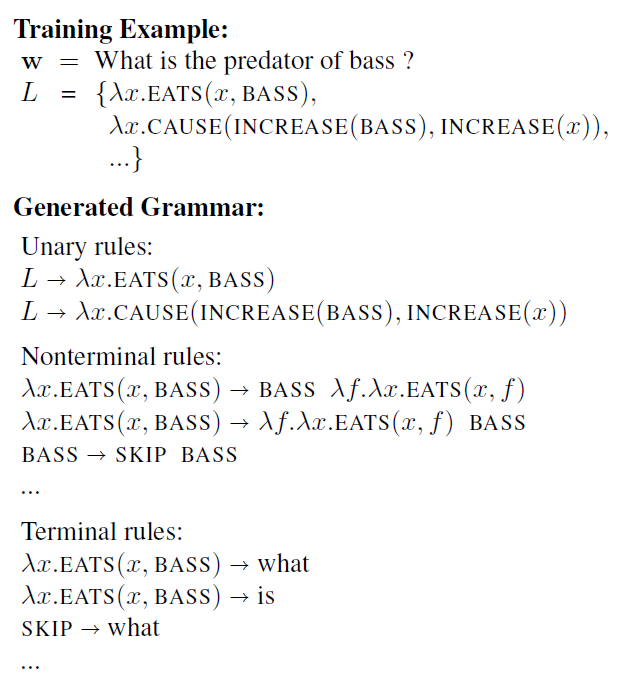
\includegraphics[width=0.48\textwidth]{rules}
\caption{The grammar generated by the algorithm from a training example}\label{fig:rules}
\end{figure}

\subsubsection{Modelling probabilities}
The generated rules from many different training examples form a grammar $G$. The replacement rules in $G$ can build a large amount of parse trees. To determine the most likely interpretation for a question, we need to know the probability of generating each unique parse tree. $P(t|L; \theta)$ denotes the probability of generating tree $t$ from $G$ with as root a given label $L$, and parameters $\theta$. This can in turn be broken down into a product of the probabilities of applying each rule in $t$. $ P(f \rightarrow g \enspace h; \theta)$ and $ P(f \rightarrow w; \theta)$ represent the probability of picking a replacement rule given the nonterminal $f$.

\begin{figure}[H]
\begin{center}
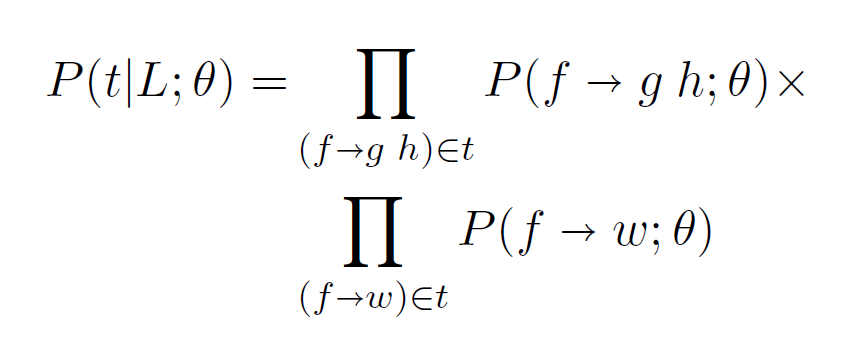
\includegraphics[width=0.4\textwidth]{prob1}
\end{center}
\label{fig:prob1}
\end{figure}

Not all of these trees build the same question, so for each specific question we're interested in all the trees with root $L$ that build a certain question $w$. This can be denoted as $P(w, t|L; \theta)$. Finally, the probability of building a question given L is:

\begin{figure}[H]
\begin{center}
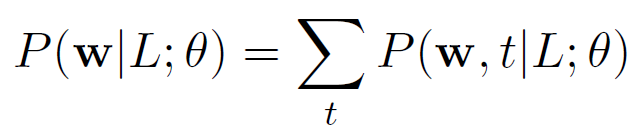
\includegraphics[width=0.3\textwidth]{coupled}
\end{center}
\label{fig:coupled}
\end{figure}

To train the model, expectation maximisation can be used. This will tweak the probabilities of applying each replacement rule in such a way that the probabilities of generating the training questions is are maximised when their labels are given. With the probabilities of applying the specific rules from grammar optimised, parser can determine the most likely parse tree by going through the building process in reverse.

\begin{figure}[H]
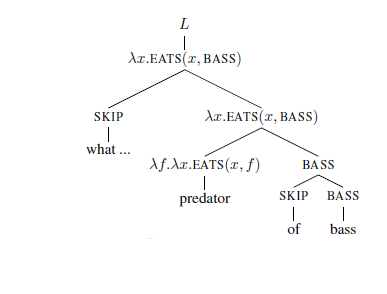
\includegraphics[width=0.48\textwidth]{parsetree}
\caption{The parse tree for the question ``What is the predator of bass?'' During training, the algorithm works from the top down to build the replacement rules. When the model is actually applied, these replacement rules are applied from the bottom up to come up with the final interpretation.}\label{fig:parsetree}
\end{figure}

\subsection{Querying the knowledge graph}
Once the meaning of the question is clear, an answer needs to be found in the knowledge base. The algorithm by Li and Clark \cite{sciencequestions} is one way to achieve that goal. After parsing the question, they extract keywords. Background knowledge is added, which results in a knowledge graph of concepts connected by the relations found in the knowledge base. These concepts are the keywords themselves, but also other related words which provide context. The questions are multiple choice, so each option is placed within that graph and connected to the other concepts. The answer that gets the highest confidence score in the knowledge graph is chosen as the solution.

\begin{figure}[H]
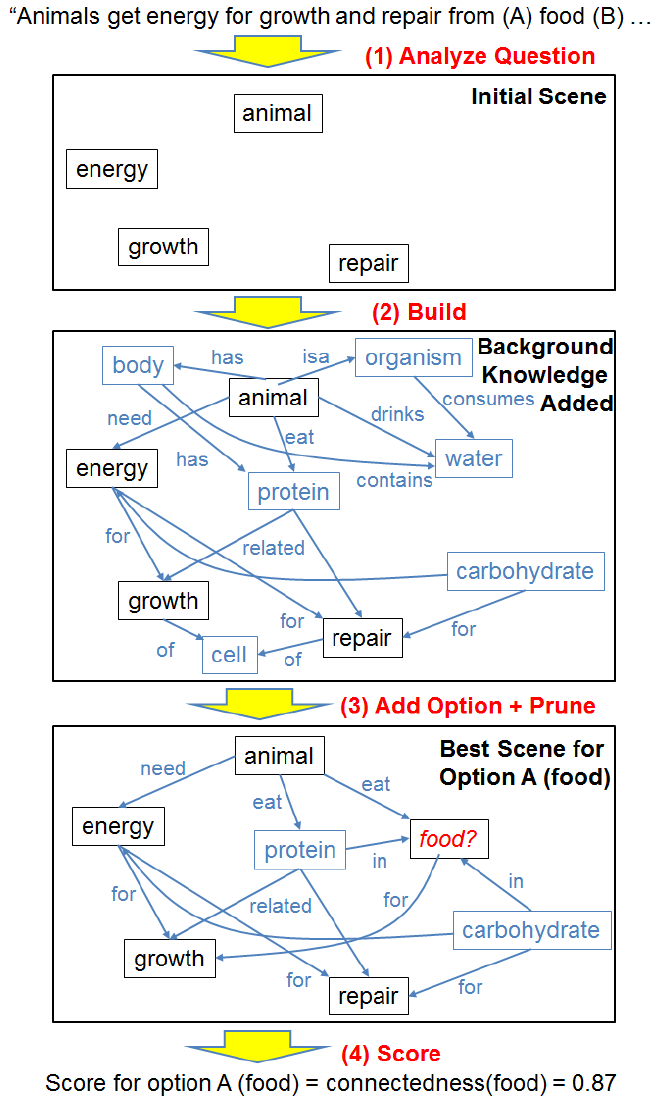
\includegraphics[width=0.48\textwidth]{graph}
\caption{An example of a question being answered using a knowledge graph.}\label{fig:parsetree}
\end{figure}





